\begin{frame}{}
    \LARGE Contrastive Learning: \textbf{Simple Framework for Contrastive Learning (SimCLR)}
\end{frame}

\begin{frame}[allowframebreaks]{SimCLR: Simple Framework for Contrastive Learning}
\begin{figure}
    \centering
    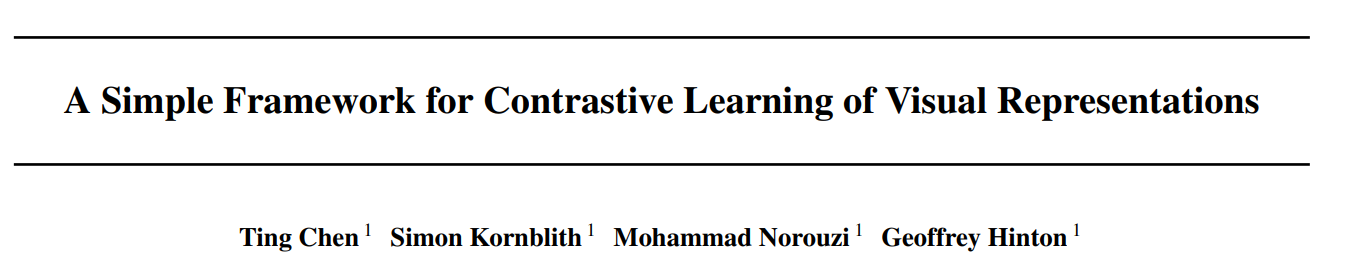
\includegraphics[width=\linewidth,height=0.9\textheight,keepaspectratio]{images/contrastive/slide_72_1_img.png}
\end{figure}

\framebreak

\textbf{What is SimCLR?}
\begin{itemize}
    \item A simple and powerful method for learning image features without labels.
    \item Uses contrastive learning:
    \begin{itemize}
        \item Pulls similar images (augmentations of the same image) closer together.
        \item Pushes different images (from different sources) further apart.
    \end{itemize}
\end{itemize}

\framebreak

\begin{figure}
    \centering
    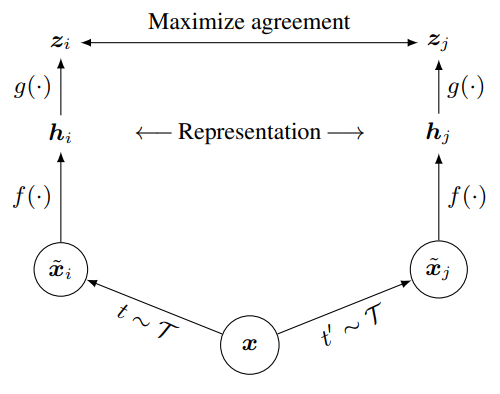
\includegraphics[width=\linewidth,height=0.9\textheight,keepaspectratio]{images/contrastive/slide_73_1_img.png}
\end{figure}

\framebreak

\textbf{Why was SimCLR created?}
\begin{itemize}
    \item Earlier contrastive learning methods needed extra tricks:
    \begin{itemize}
        \item Memory banks to store negative examples.
        \item Special momentum encoders.
    \end{itemize}
    \item SimCLR avoids these by:
    \begin{itemize}
        \item Using very large batch sizes.
        \item Always having plenty of negative examples in each batch.
    \end{itemize}
    \item This makes SimCLR simpler and easier to train.
\end{itemize}

\framebreak

\textbf{How does SimCLR work?}
\begin{itemize}
    \item \textbf{Augmentation pipeline:}
        \begin{itemize}
            \item Each image is randomly cropped.
            \item Color is changed.
            \item Sometimes blurred.
            \item This creates two different views of the same image.
        \end{itemize}
    \framebreak
    \item \textbf{Encoder + Projection Head:}
        \begin{itemize}
            \item Both views go through a neural network encoder ($f(\cdot)$).
            \item Then, they pass through a small MLP called the projection head ($g(\cdot)$).
            \item This gives the final representations.
        \end{itemize}
    \framebreak
    \item \textbf{Contrastive Loss (NT-Xent):}
        \begin{itemize}
            \item The model pulls together representations of two views of the same image.
            \item It pushes apart representations of different images.
            \item The loss function is:
            \[
            \ell_{i,j} = -\log \frac{\exp(\text{sim}(z_i, z_j)/\tau)}{\sum_{k \neq i} \exp(\text{sim}(z_i, z_k)/\tau)}
            \]
            \item $\text{sim}(z_i, z_j)$ is the similarity between two representations.
            \item $\tau$ is a temperature parameter.
        \end{itemize}
\end{itemize}

\framebreak

\begin{figure}
    \centering
    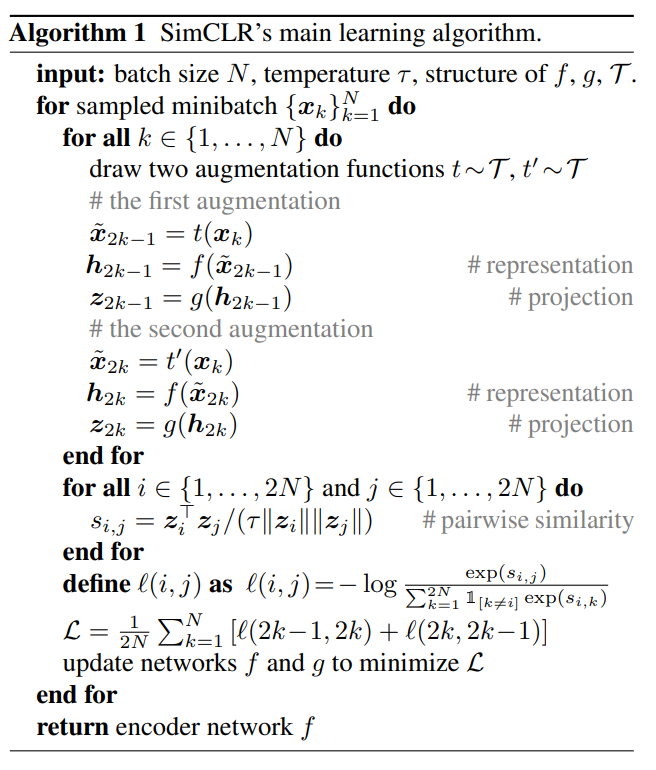
\includegraphics[width=\linewidth,height=0.9\textheight,keepaspectratio]{images/contrastive/slide_74_1_img.png}
\end{figure}

\framebreak

\begin{figure}
    \centering
    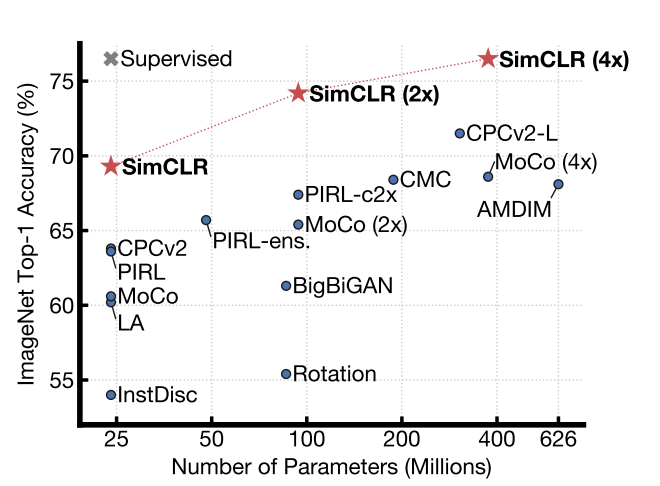
\includegraphics[width=\linewidth,height=0.9\textheight,keepaspectratio]{images/contrastive/slide_75_1_img.png}
\end{figure}

\framebreak

\begin{figure}
    \centering
    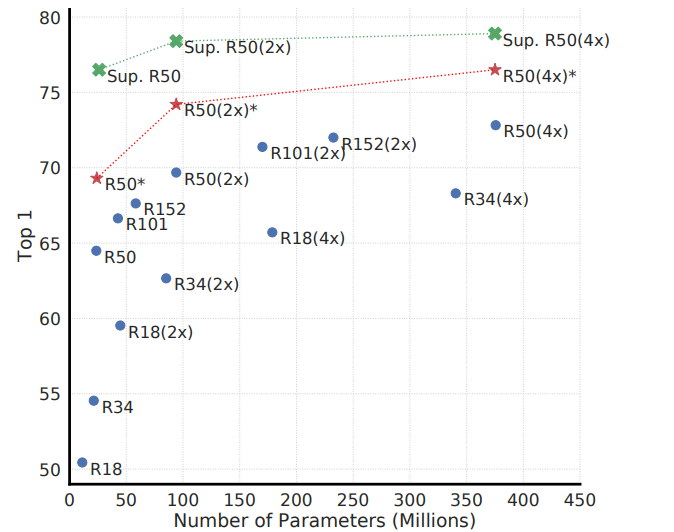
\includegraphics[width=\linewidth,height=0.9\textheight,keepaspectratio]{images/contrastive/slide_76_1_img.png}
\end{figure}

\framebreak

\textbf{What did we learn from SimCLR?}
\begin{itemize}
    \item Using strong data augmentations is really important for learning good features.
    \item Adding a nonlinear projection head (the MLP) helps the model learn better representations.
    \item SimCLR needs large batch sizes, which means it requires a lot of computing power.
\end{itemize}
\end{frame}



\begin{frame}[allowframebreaks]{MoCov2 vs. SimCLR}
\begin{figure}
    \centering
    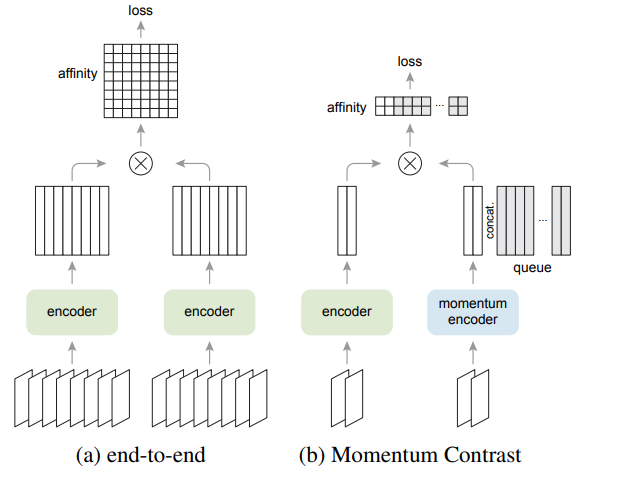
\includegraphics[width=\linewidth,height=0.9\textheight,keepaspectratio]{images/contrastive/slide_77_1_img.png}
\end{figure}

\framebreak

\begin{figure}
    \centering
    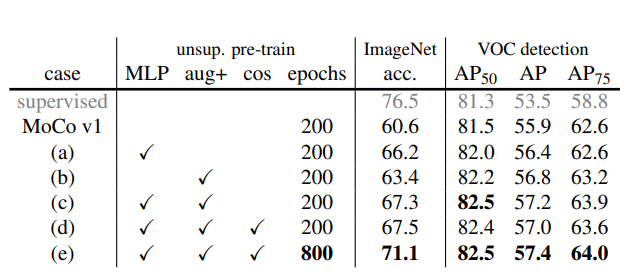
\includegraphics[width=\linewidth,height=0.9\textheight,keepaspectratio]{images/contrastive/slide_78_1_img.png}
\end{figure}

\framebreak

\begin{figure}
    \centering
    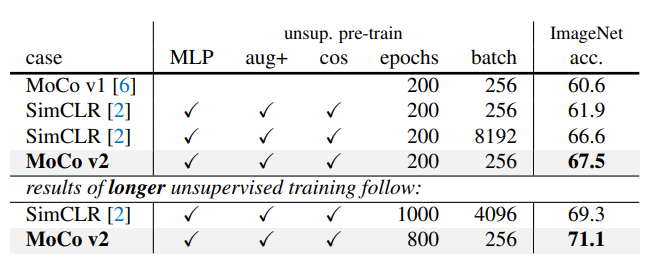
\includegraphics[width=\linewidth,height=0.9\textheight,keepaspectratio]{images/contrastive/slide_79_1_img.png}
\end{figure}

\end{frame}